\documentclass[10pt,twocolumn,letterpaper]{article}

\usepackage{cvpr}
\usepackage{times}
\usepackage{epsfig}
\usepackage{graphicx}
\usepackage{amsmath}
\usepackage{amssymb}

% Include other packages here, before hyperref.

% If you comment hyperref and then uncomment it, you should delete
% egpaper.aux before re-running latex.  (Or just hit 'q' on the first latex
% run, let it finish, and you should be clear).
\usepackage[breaklinks=true,bookmarks=false,draft]{hyperref}

\cvprfinalcopy % *** Uncomment this line for the final submission

\def\cvprPaperID{----} % *** Enter the CVPR Paper ID here
\def\httilde{\mbox{\tt\raisebox{-.5ex}{\symbol{126}}}}

% Pages are numbered in submission mode, and unnumbered in camera-ready
%\ifcvprfinal\pagestyle{empty}\fi
\setcounter{page}{1}
\begin{document}

%%%%%%%%% TITLE
\title{Chinese Character Style Transfer with conditional GAN}

\author{Ho Kei Cheng\\
Hong Kong University of Science and Technology\\
{\tt\small hkchengad@connect.ust.hk}
}

\maketitle
%\thispagestyle{empty}

%%%%%%%%% ABSTRACT
\begin{abstract}
	Image generation and style transfer have became a hot topic in research. 
	Generative Adversarial Networks (GANs) have been used to solve a lot of image generation
	problems. We here present an attempt at using GANs to perform style transfer by formulating
	it as an image generation problem on Chinese characters. Unlike most previous works, 
	our method does not focus on a singleton image transform. It learns how to transform an image
	to a unseen style by looking at font samples from the new style. Thus, no re-training is required
	to deal with novel fonts.
\end{abstract}

%%%%%%%%% BODY TEXT
\section{Introduction}
The advancement of deep convolutional neural networks (DCNNs) has enabled computers
to better understand images at different abstraction levels. 
They are able to transfer the low level features like storkes and color
from an image to another, or even to generate images based on description.
Eariler studies on neural style transfer tries to minimize the difference 
between both the style and content of the source and target images using 
features from DCNN. \cite{DBLP:journals/corr/JohnsonAL16} \cite{Authors04} \cite{Authors03}

Recently, Generative Adversarial Networks (GANs) have also been used on
style transfer and image generation problems and have achieved success. GANs include both a generator and a discriminator. By imposing an additional discriminator as a guidance to the generator, GANs tend to generate more realistic images.
GANs include a generator and a discriminator having the objective function
\begin{align*}
\mathcal{L}_{GAN}(G, D)=&\mathbb{E}_{y}[\log(D(y))] +  \\&\mathbb{E}_{x,z}[\log(1-D(G(x,z))))]
\end{align*}
where the generator $G$ tries to minimize this objective while $D$ tries to maximize it. \cite{DBLP:journals/corr/RadfordMC15}

In this paper, we propose a style transfer GAN that can be used on multiple, unseen styles and content. The network is designed to extract content information and style information separately early on and combine them at a later stage. 

We focus on style transfer for Chinese fonts. Traditionally it is difficult to design new Chinese fonts as there are more than 4,000 commonly used Chinese characters and all of them have to be designed manually \cite{Authors02}. Our method aims to automatically generate the entire character set including thousands of characters given a few style references.

%------------------------------------------------------------------------
\section{Related Work}

\subsection{Image translation}
Image-to-image translation learns from paired images and attempts to establish the transformation from one image domain to another. It includes generating color images from grayscale images or converting day scene to night scene. Previous work like conditional GAN (cGAN) \cite{Authors01}, pix2pix\cite{DBLP:journals/corr/IsolaZZE16} and cycle-consistent adversarial network (CycleGAN)\cite{DBLP:journals/corr/ZhuPIE17} have shown appealing results in image translation. However, all of them are fixed to learn only one transformation at a time. To perform a new transform, the network must be retrained.

\subsection{Font Style Transfer}
A number of previous works have also studied the character style transfer process. "From A to Z" perform style transfer on English characters using variational autoencoder (VAE) \cite{DBLP:journals/corr/UpchurchSB16}. A online project zi2zi borrows idea from pix2pix, using GAN with encoder-decoder and the U-net structure in the generator to perform font generation in a latent space created by some fixed font styles. Another work AEGN also uses GAN to generate calligraphy using a standard font directly \cite{DBLP:journals/corr/LyuBYZHL17}. A more recent and aligned work is the EMD model, which separate the content and style representation using two distinct encoders \cite{DBLP:journals/corr/abs-1711-06454}. 


%------------------------------------------------------------------------
\section{Method}
Our model consists of two parts: \textit{Generator} and \textit{Discriminator}. The generator will be feed with reference context and reference style, trying to generate the character in the said context with the given style. The disciminator then tries to distinguish generated characters with ground truths.

\begin{figure*}
	\begin{center}
		\fbox{\rule{0pt}{2in} \rule{.9\linewidth}{0pt}}
	\end{center}
	\caption{The network structure}
	\label{fig:short}
\end{figure*}


\subsection{Generator}
The generator consists of two encoders and a decoder. The two encoders are \textit{Style Encoder} and \textit{Context Encoder} respectively. All the reference context will be concatenated together and fed into the context encoder. The styles will be fed one by one into the style encoder. 

After all the contexts and styles have been encoded, they are concatenated together and passed to the decoder network. The output from the decoder network is the generated result.

\subsubsection{Encoder}
Both the \textit{Style Encoder} and \textit{Context Encoder} consist of layers of $3x3Convolution - BatchNorm - ReLU$. Max-poolings are used to reduce the dimension of the original $64*64$ input to $8*8$ encoded output. 

\subsubsection{Decoder}
To enchance the quaility of generated images, transposed convolutions (also known as deconvolution) are used to upsample the encoded context and style reference, as suggested by DCGAN\cite{DBLP:journals/corr/RadfordMC15}. The decoder network is a transposed version of the encoder, except that transposed convolution with input padding of 2 and output padding of 1 has replaced max-poolings.

There are U-Net\cite{DBLP:journals/corr/RonnebergerFB15} like structure which connect the encoder and decoder together with skip-connection to preverse some of the lost information in max-pooling.

\subsection{Discriminator}
There are two small networks in the discriminator. They are the  \textit{Context Discriminator} and \textit{Style Discriminator} respectively. The context discriminator takes the image-to-be tested with the context reference to determine its realness in terms of context. The style discriminator take the style reference instead, and compare realness in terms of style. Their results are averaged to obtain overall discriminator score.

\subsection{Losses}
We have used the binary cross entropy loss to update the discriminator, guiding it to output 1 for ground truth images and 0 for generated images. 

For the generator, both binary cross entropy loss and L1 loss is used as suggested by pix2pix. The binary cross entropy loss guides the generator to output images that the discriminator will give high score, i.e. to fool the discriminator. The L1 loss compare the generator's output and the ground truth image.

\section{Result}
The network can successfully generate readable characters that have similar low-level features as ground truths. However, there are a few issues:

\begin{enumerate}
	\item Thins stroke might be missing.
	\item The generated image looks "dirty", i.e. has noises.
	\item It failed to learn high level features like spacing between strokes.
\end{enumerate}


\begin{figure}[t]
	\begin{center}
		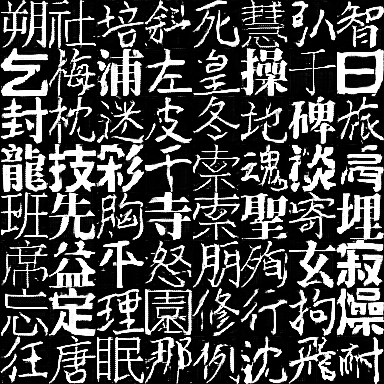
\includegraphics[width=0.8\linewidth]{385gen.png}
		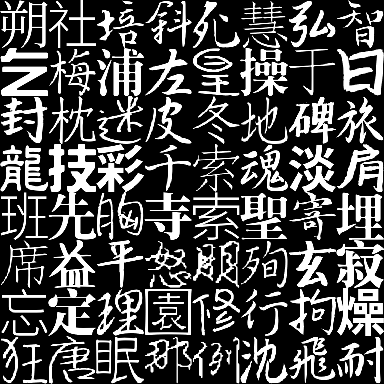
\includegraphics[width=0.8\linewidth]{385gt.png}
		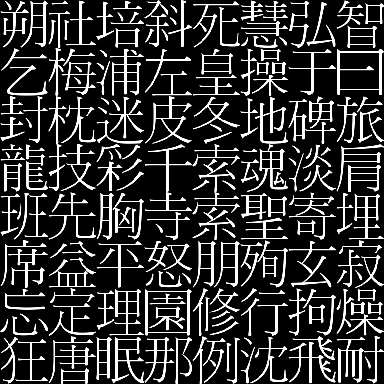
\includegraphics[width=0.8\linewidth]{385r1.png}
	\end{center}
	\caption{Generating different characters in different fonts in a single batch. Top to bottom: Generated characters, ground truth and one of the context reference}
	\label{fig:long}
	\label{fig:onecol}
\end{figure}

\begin{figure}[t]
	\begin{center}
		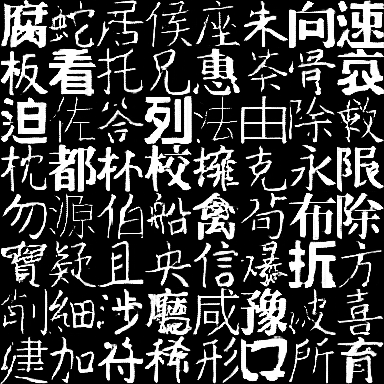
\includegraphics[width=0.8\linewidth]{380gen.png}
		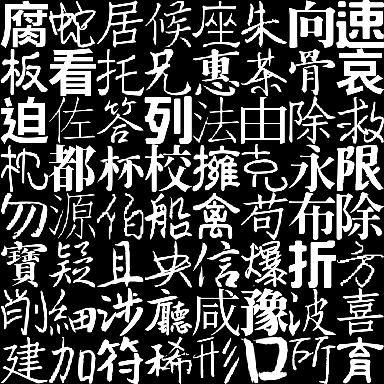
\includegraphics[width=0.8\linewidth]{380gt.png}
		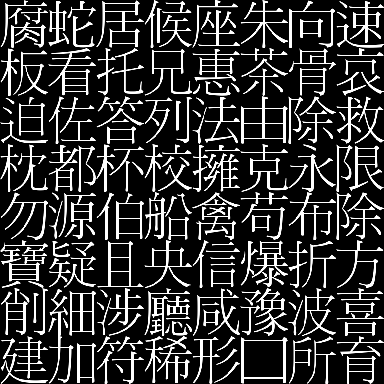
\includegraphics[width=0.8\linewidth]{380r1.png}
	\end{center}
	\caption{Another result. Top to bottom: Generated characters, ground truth and one of the context reference}
	\label{fig:long}
	\label{fig:onecol}
\end{figure}

\section{Implementation and data}
The model is implementated with PyTorch. It is trained with SGD with learning rate $0.001$, momentum of $0.9$ and batch size $64$ for 400 epochs. The training took 15 hours on a GTX970.

31 fonts are obtained onlined. 23 of them are used in style reference training, 5 of them used as context reference and the rest act as test set. 1702 commonly used Chinese characters are picked to be used in training.

Note that different fonts can have significant difference in size and position even when the same font size and origin is used. Preprocessing is done so that the bounding box of each character aligns.

{\small
\bibliographystyle{ieee}
\bibliography{egbib}
}

\end{document}
